Consider the pinned beam with constant cross section and mass distribution shown below. The beam is supported at one end by a pinned joint. For this exercise, you can assume the beam is stationary $(\boldsymbol{a}=\boldsymbol{\alpha}=0, \boldsymbol{v}=\boldsymbol{\dot{\theta}}=0)$

\begin{center}
    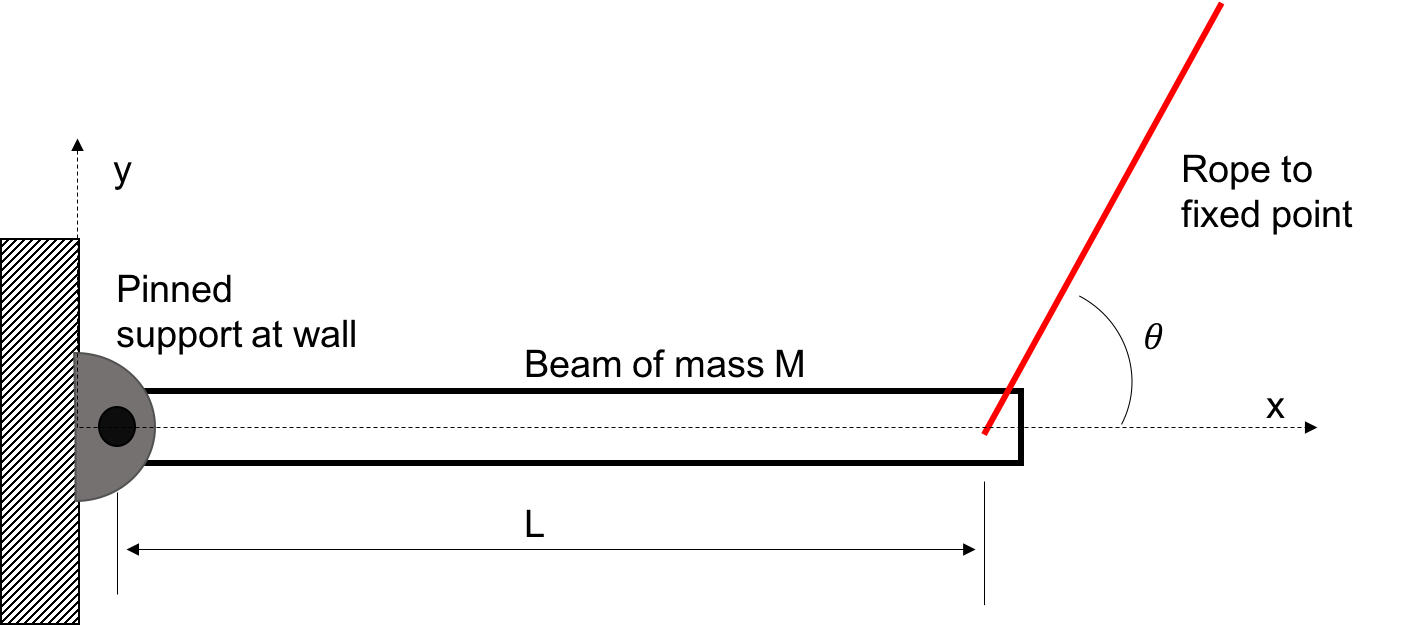
\includegraphics[width=0.75\textwidth]{img/fig24_1.png}
\end{center}

When drawing a free body diagram for the pinned beam, which body should you isolate?

\begin{solution}
    I would isolate the beam.
\end{solution}
